\documentclass{beamer}
\mode<presentation> {
\usetheme{Madrid}
\setbeamercovered{invisible}
\setbeamertemplate{navigation symbols}{} 
}


% Packages
\usepackage[utf8]{inputenc}
\usepackage{graphicx}
\usepackage{default}
\usepackage{bbding}


% Some heading
\logo{\includegraphics[height=1.2cm]{images/unipd.png}}
\title[sgap]{sgap - Scala Genetic Algorithm Package}
\author{Marco Zanella}
\institute[University of Padova]{
 University of Padova \\
 \medskip
 {\emph{marco.zanella.9@studenti.unipd.it}}
}
\date{\today}



\begin{document}
%%%%%%%%%%%%%%%%%%%%%%%%%%%%%%%%%%%%%%%%%%%%%%%%%%%%%%%%%%%%%%%%%%%%%%%%
% Title
\begin{frame}
\titlepage
\end{frame}


%%%%%%%%%%%%%%%%%%%%%%%%%%%%%%%%%%%%%%%%%%%%%%%%%%%%%%%%%%%%%%%%%%%%%%%%
% Table of contents
\begin{frame}{Table of Contents}
\tableofcontents
\end{frame}



%%%%%%%%%%%%%%%%%%%%%%%%%%%%%%%%%%%%%%%%%%%%%%%%%%%%%%%%%%%%%%%%%%%%%%%%
% Introduction
\section{Introduction}
\begin{frame}{Introduction}
  The goal of this work is to stress Scala's features on \emph{real} scenarios:
  \begin{description}
    \item [Genetic Algorithms] to exploit Object-Oriented features
    \item [Greedy Algorithms] to exploit functional features
  \end{description}
  And with \emph{concrete} use cases:
  \begin{itemize}
    \item The Traveling Salesman Problem
    \item The Knapsack 1-0 problem
  \end{itemize}
\end{frame}


% Scala
\subsection{Scala}
\begin{frame}{Introduction - Scala}
  \begin{columns}[onlytextwidth]
    \begin{column}{0.6\textwidth}
      \includegraphics[width=0.95\textwidth]{images/scala-tree}
    \end{column}
    \begin{column}{0.4\textwidth}
     Modern, multi-paradigm programming language:
     \begin{itemize}
      \item Object-Oriented
      \item Functional
      \item Statically Typed
      \item Extensible
     \end{itemize}
     Famous for its actor-based concurrency model, it offers more
     interesting features.
    \end{column}
  \end{columns}
\end{frame}


% Genetic algorithms
\subsection{Scenarios}
\begin{frame}{Introduction - Genetic Algorithms}
  Search heuristic inspired by natural selection (Charles Darwin).
  \begin{center}
   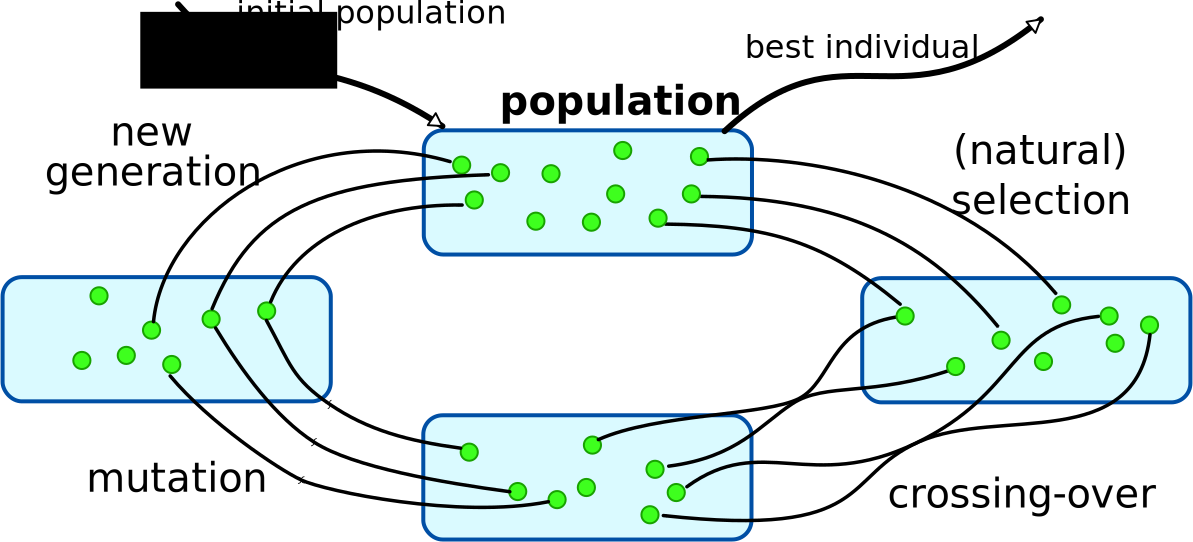
\includegraphics[width=0.75\textwidth]{images/genetic-algorithms}
  \end{center}
  GAs use \emph{no or little knowledge} about the properties of the problem.
  \footnotesize{
    \begin{thebibliography}{99}
      \bibitem[Label5, 1998]{key1} Marek Obitko
      \newblock Introduction to Genetic Algorithms
    \end{thebibliography}
  }
  %http://www.obitko.com/tutorials/genetic-algorithms/index.php
\end{frame}


% Greedy algorithms
\begin{frame}{Introduction - Greedy Algorithms}
  Simple heuristics which make a locally optimal choiche at each stage.
  \begin{itemize}
    \item optimal solution/termination is not guaranteed (except for matroids)
    \item very fast
    \item usually good solutions
  \end{itemize}
  \begin{center}
    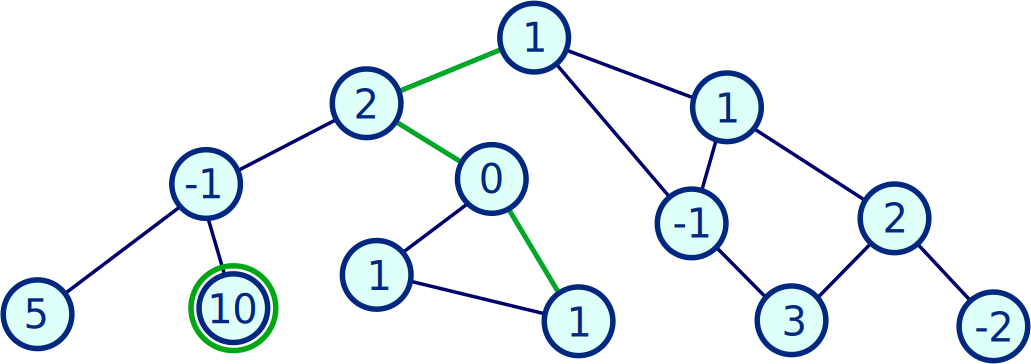
\includegraphics[height=0.4\textheight]{images/greedy}
  \end{center}
  Greedy algorithms require little knowledge about the problem.
\end{frame}



%%%%%%%%%%%%%%%%%%%%%%%%%%%%%%%%%%%%%%%%%%%%%%%%%%%%%%%%%%%%%%%%%%%%%%%%
% Core concepts
\section{Core concepts}
\begin{frame}{Core concepts}
  A lot of (hard) mathematics behind Genetic Algorithms:
  \begin{columns}[onlytextwidth]
    \begin{column}{0.5\textwidth}
      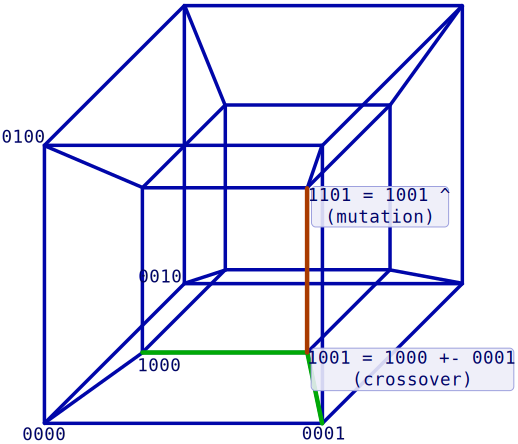
\includegraphics[width=0.95\textwidth]{images/hypercube}
    \end{column}
    \begin{column}{0.5\textwidth}
     \begin{itemize}
      \item search space as hypercubes
      \item axioms of closure under crossover and mutation
      \item convergence
      \item ...
     \end{itemize}
     Also negative results such as the \emph{No Free Lunch Theorem} must
     be understood.
    \end{column}
  \end{columns}
  \footnotesize{
    \begin{thebibliography}{99}
      \bibitem[Label5, 1998]{key6} Thomas Weise
      \newblock Global Optimization Algorithms
    \end{thebibliography}
  }
\end{frame}


% Why Scala?
\subsection{Why Scala?}
\begin{frame}{Core concepts - Why scala?}
  Many interesting benefits:
  \begin{itemize}
   \item Type safety
   \item Type inference (much less verbose than Java)
   \item Object Oriented... (unlike Haskell)
   \item ...and functional (unlike Java and C++)
   \item Traits (better than PHP's or Ruby's)
   \item \tiny (To try out something new...)
  \end{itemize}
  No real disadvantages so far, but:
  \begin{itemize}
   \item Slow compile phase (solved by incremenetal compilation)
   \item Some features not (yet) available
  \end{itemize}

\end{frame}


% Test cases
\subsection{Test cases}
\begin{frame}{Core concepts - Test cases}
  Genetic Algorithms are commonly applied to a variety of fields.
  Programs based on combinatorial problems are common killer applications.
  \begin{center}
   \includegraphics[width=0.9\textwidth]{images/test-cases}
  \end{center}
  Both the \emph{Traveling Salesman Problem (TSP)} and the \emph{Knapsack 1-0 Problem}
  are well-known \emph{NP-hard} problems.
\end{frame}


\begin{frame}{Core concepts - Test cases}
  \begin{description}
    \item[Knapsack 1-0] Which are the best items to put into a limited size knapsack? (no more than 1 of each item!)
    \item[TSP] Given a set of cities, which is the shortest path which goes though them all?
  \end{description}
  Differences between Knapsack and TSP make them suitable test cases:
  \begin{center}
    \begin{tabular}{||l|l||}
      \hline
      Knapsack 1-0                     & TSP\\
      \hline
      \hline
      size of solution not know        & size of solution know\\
      \hline
      maximize ($\Sigma$ of values)    & minimize ($\Sigma$ of distances)\\
      \hline
      constraint ($\Sigma$ of weights) & unconstrained\\
      \hline
      order of items does not matter   & order of items matters\\
      \hline
    \end{tabular}
  \end{center}
\end{frame}




%%%%%%%%%%%%%%%%%%%%%%%%%%%%%%%%%%%%%%%%%%%%%%%%%%%%%%%%%%%%%%%%%%%%%%%%
% Code implementation
\section{Code implementation}
\begin{frame}{Code implementation}
  \begin{columns}[onlytextwidth]
    \begin{column}{0.6\textwidth}
      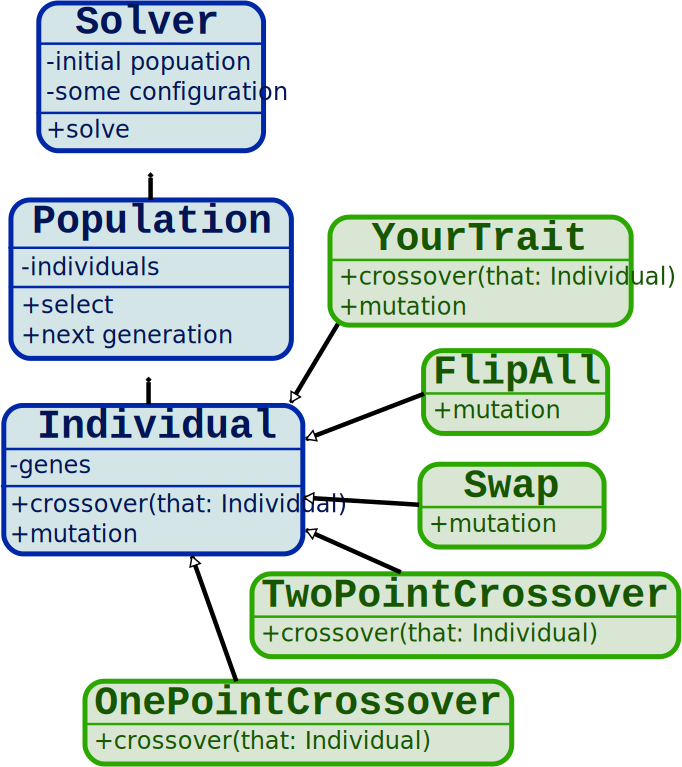
\includegraphics[width=0.95\textwidth]{images/uml}
    \end{column}
    \begin{column}{0.4\textwidth}
      Functional and OO can live together:
      \begin{description}
	\item [GA] Object Oriented
	\item [Greedy] functional
      \end{description}
      Greedy solutions as initial individuals for GAs.
      \footnotesize{
	\begin{thebibliography}{99}
	  \bibitem[Label5, 2014]{key2} Patrick R. Nicolas
	  \newblock Scala for Machine Learning
	\end{thebibliography}
      }
    \end{column}
  \end{columns}
\end{frame}


% Strategies
\subsection{Strategies}
\begin{frame}{Code implementation - Strategies}
  \begin{center}
    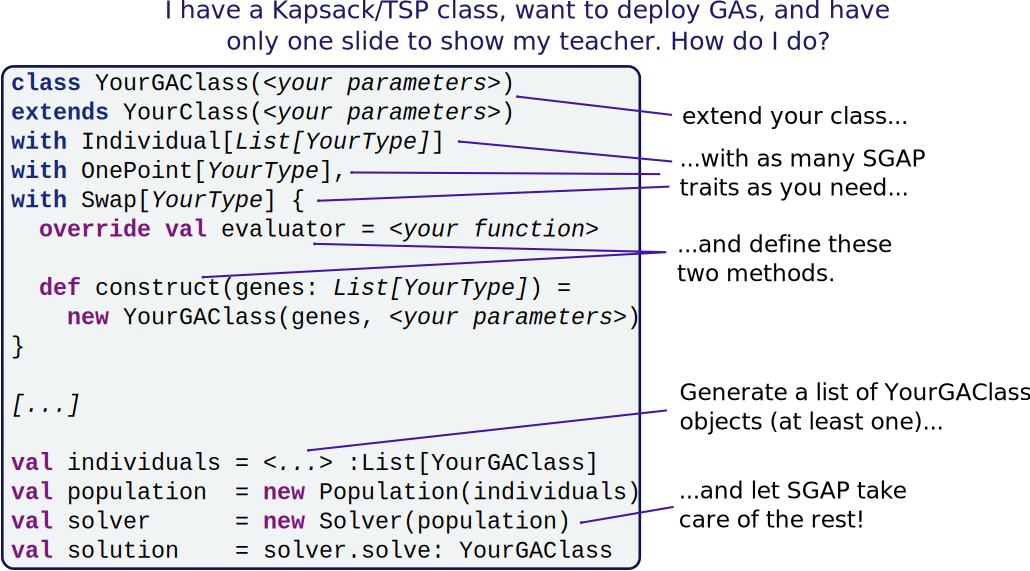
\includegraphics[width=0.9\textwidth]{images/real-code}
  \end{center}
\end{frame}


\begin{frame}{Code implementation - Strategies}
  \begin{center}
    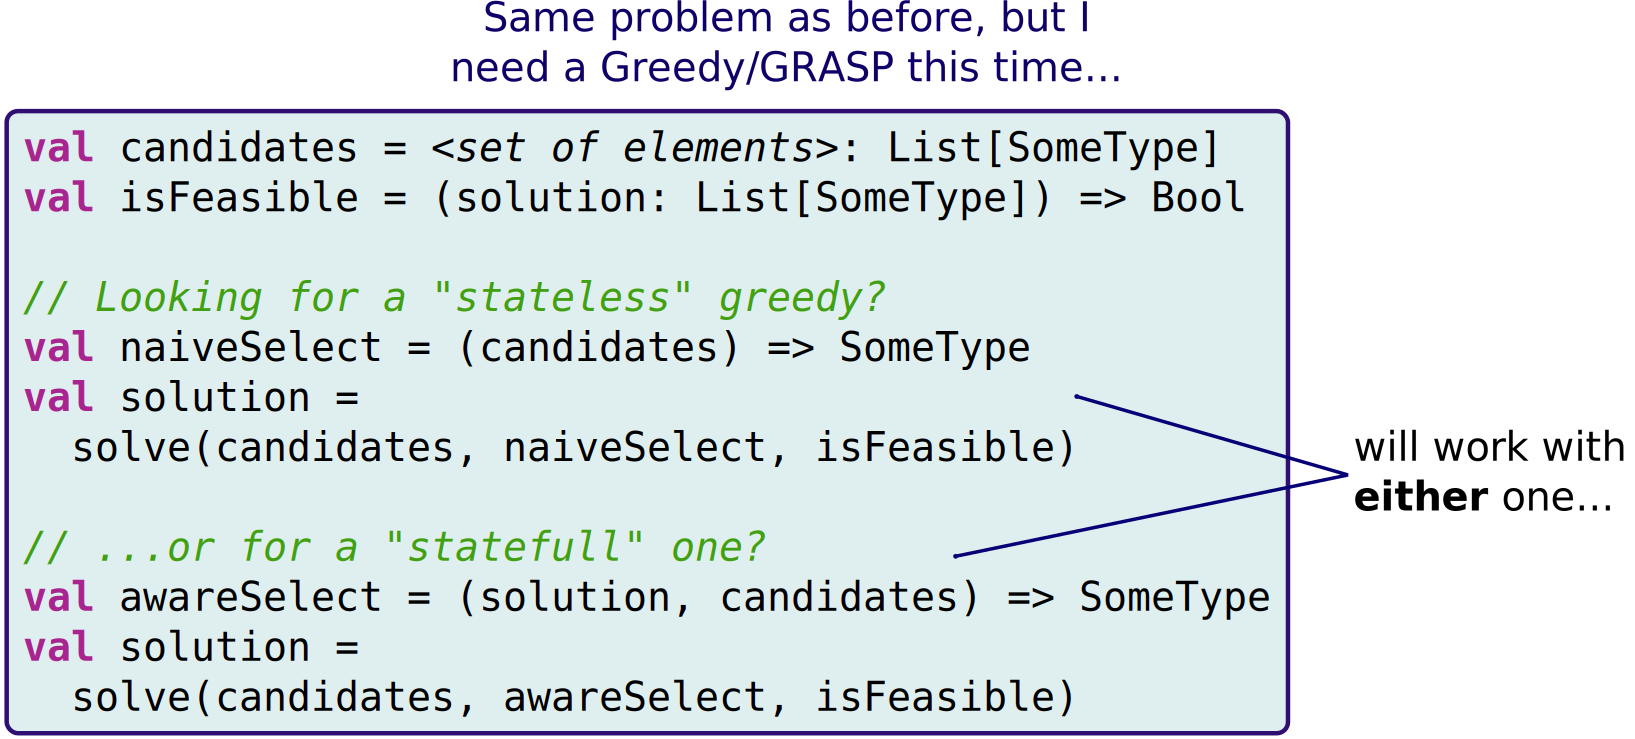
\includegraphics[width=0.9\textwidth]{images/real-code-greedy}
  \end{center}
\end{frame}



% Result analysis
\subsection{Result analysis}
\begin{frame}{Code implementation - Flaws}
  There are still \emph{reasonable and desirable} features not available:
  \begin{center}
    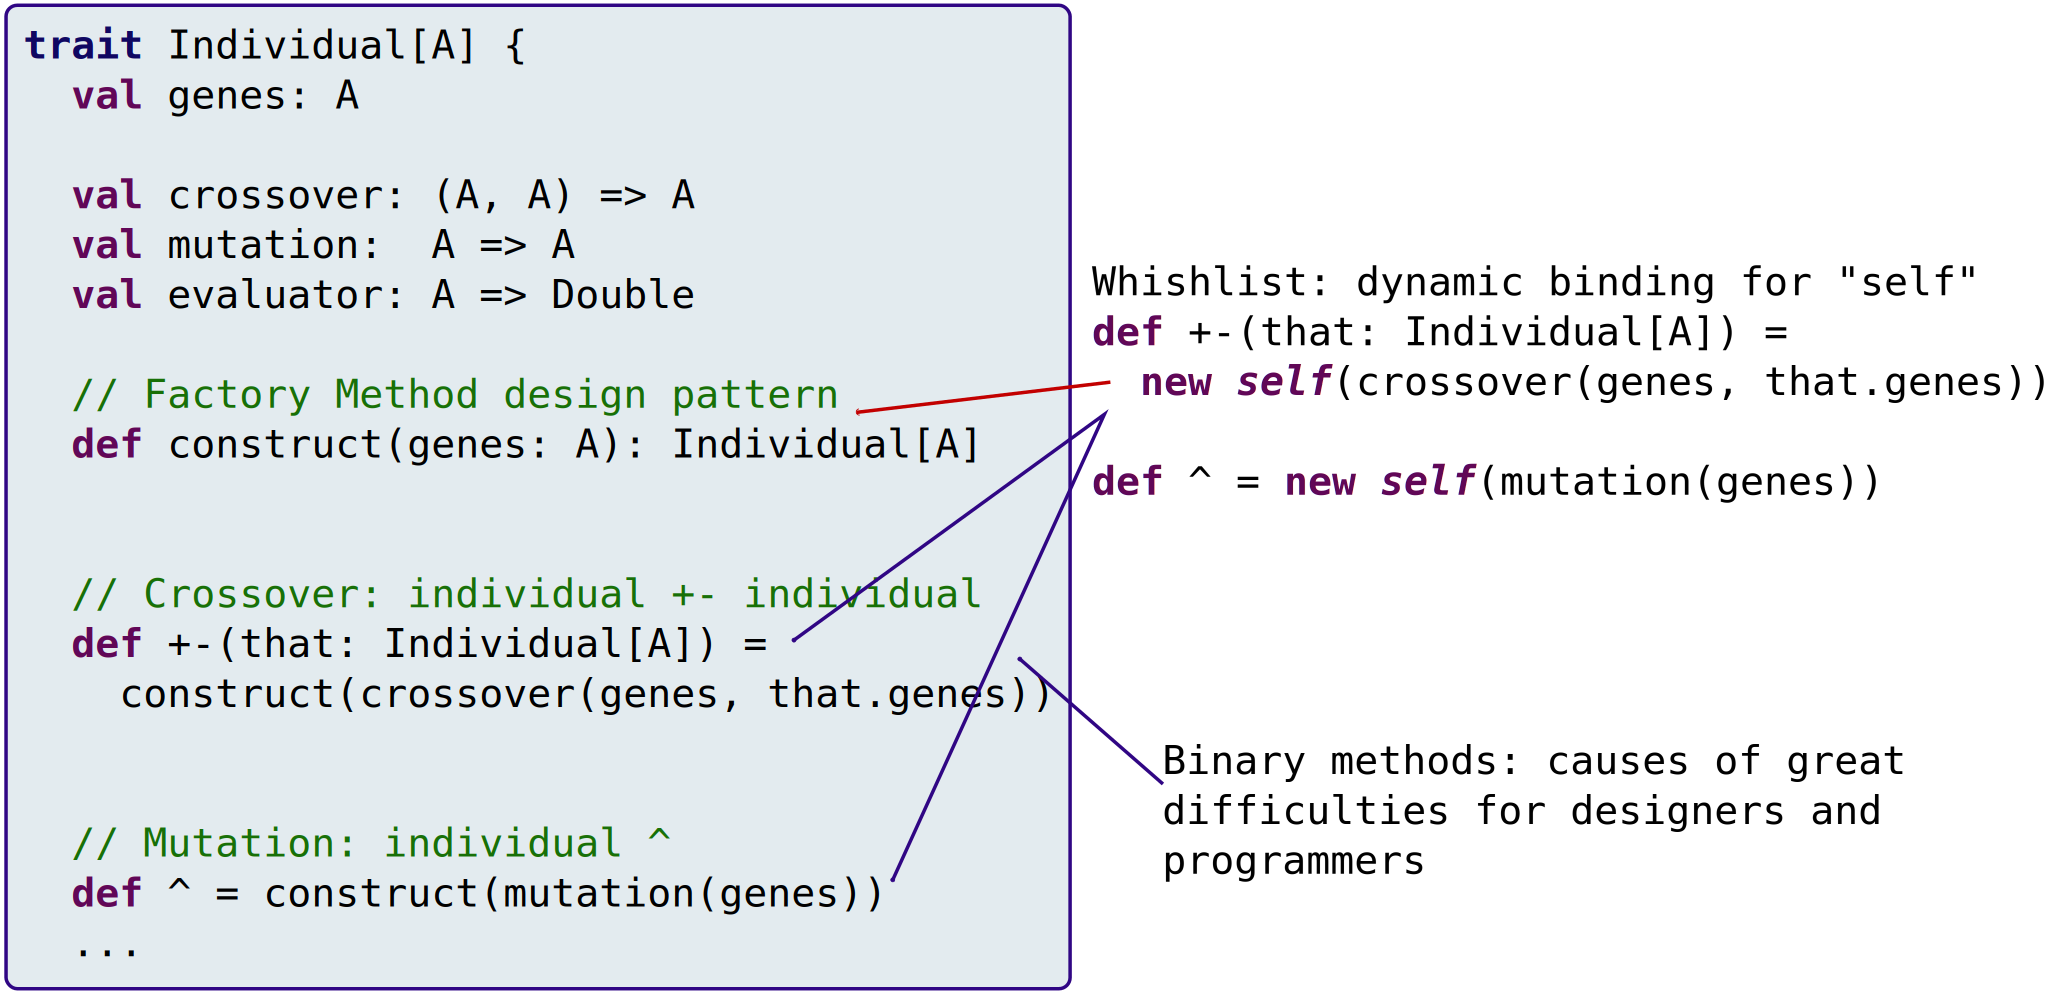
\includegraphics[width=0.9\textwidth]{images/ga-flaws}
  \end{center}
  \footnotesize{
    \begin{thebibliography}{99}
      \bibitem[Label5, 2014]{key3} Luca Cardelli et al.
      \newblock On Binary Methods
    \end{thebibliography}
  }
\end{frame}



%%%%%%%%%%%%%%%%%%%%%%%%%%%%%%%%%%%%%%%%%%%%%%%%%%%%%%%%%%%%%%%%%%%%%%%%
% Comparison with other works
\section{Similar works}
\begin{frame}{Similar works}
  There are no notable Scala works with the same goal as SGAP.
  
  Similar works include:
  \begin{description}
    \item[Java Genetic Algorithms Package] same goal, similar language
    \item[Scala for Machine Learning] similar goal, same language
  \end{description}
  SGAP (tries to) take the best out of the two.
\end{frame}


% JGAP
\subsection{JGAP}
\begin{frame}{Similar works - JGAP}
  \begin{center}
    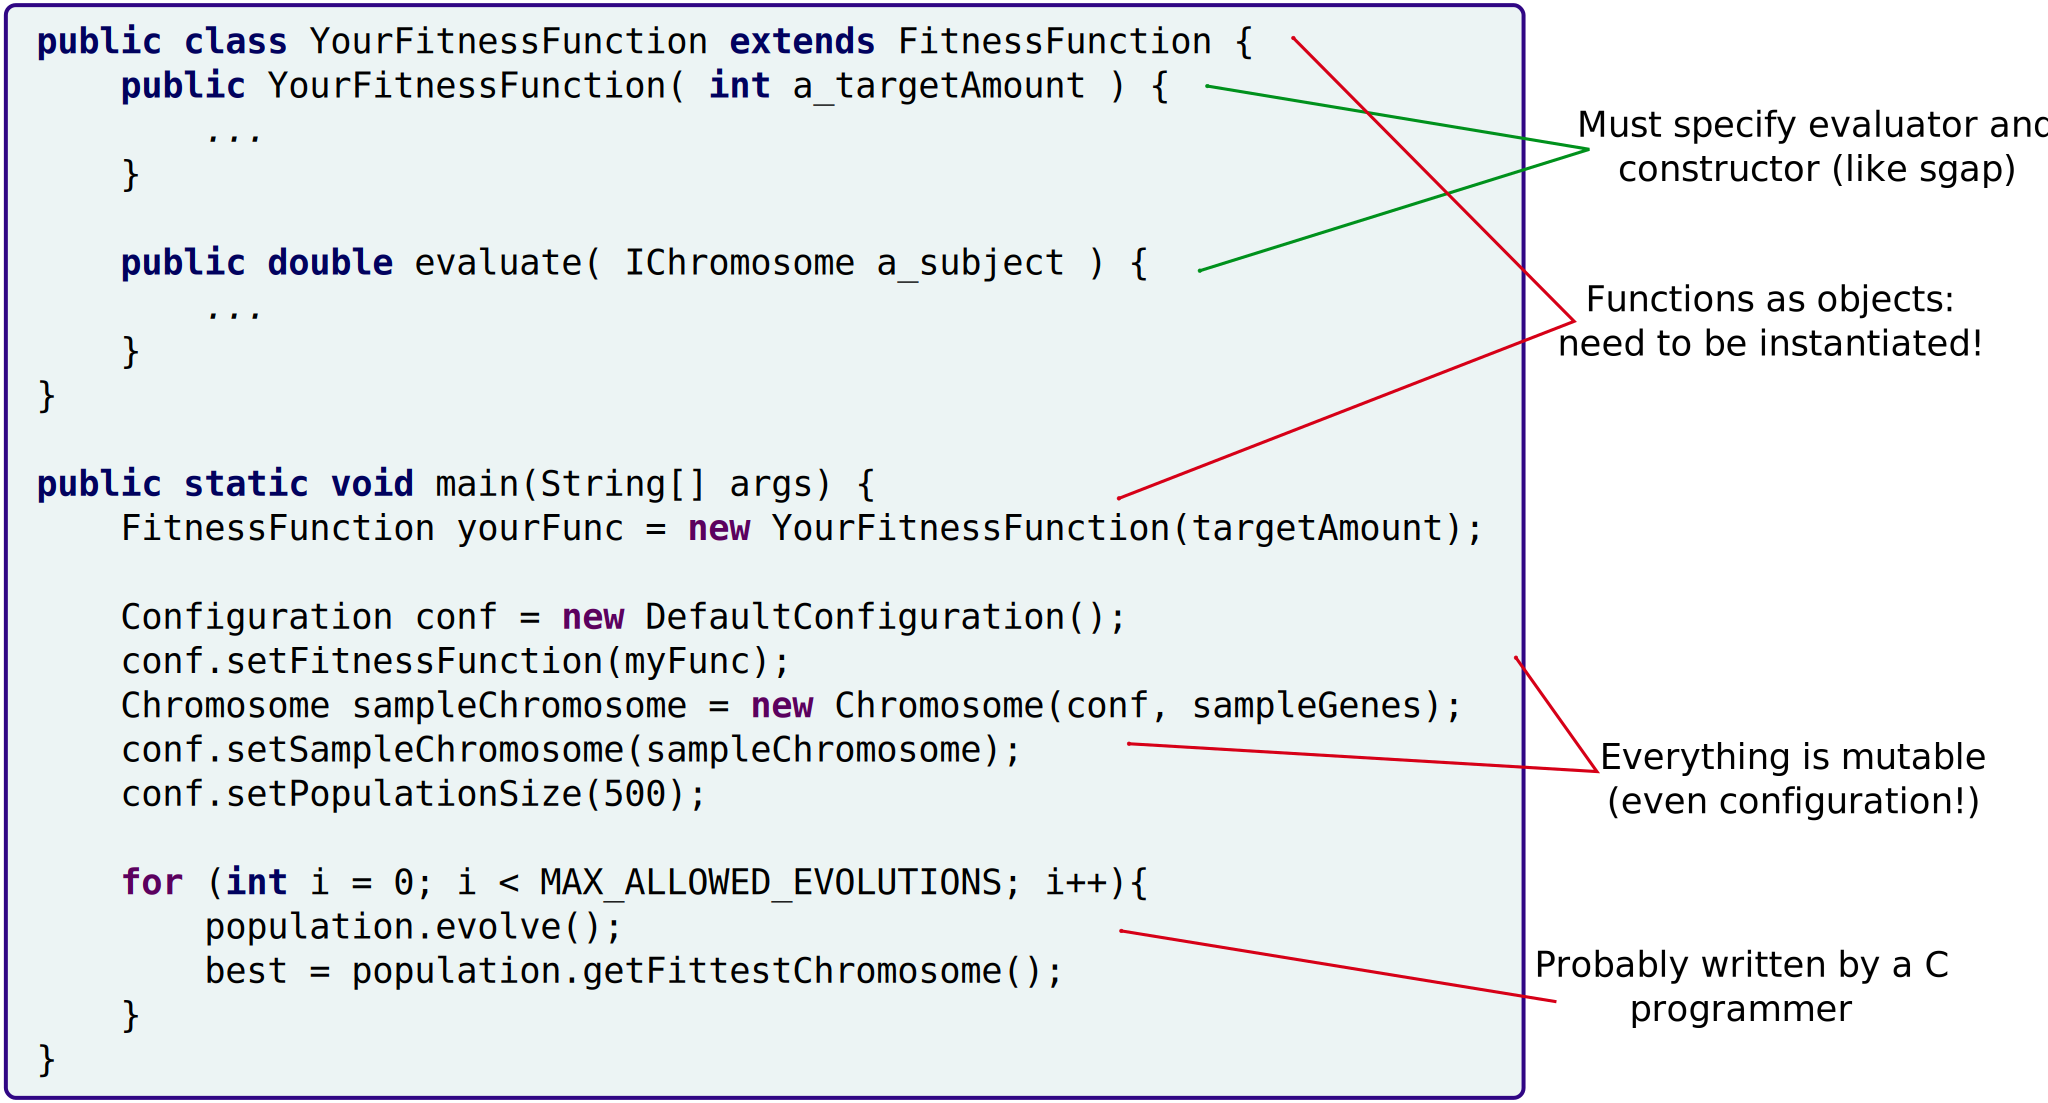
\includegraphics[width=0.9\textwidth]{images/jgap}
  \end{center}
  \footnotesize{
    \begin{thebibliography}{99}
      \bibitem[Label5, 2014]{key4} JGAP documentation
      \newblock http://jgap.sourceforge.net/
    \end{thebibliography}
  }
\end{frame}


% Scala for machine learning
\subsection{Scala for Machine Learning}
\begin{frame}{Similar works - Scala for Machine Learning}
 \begin{center}
    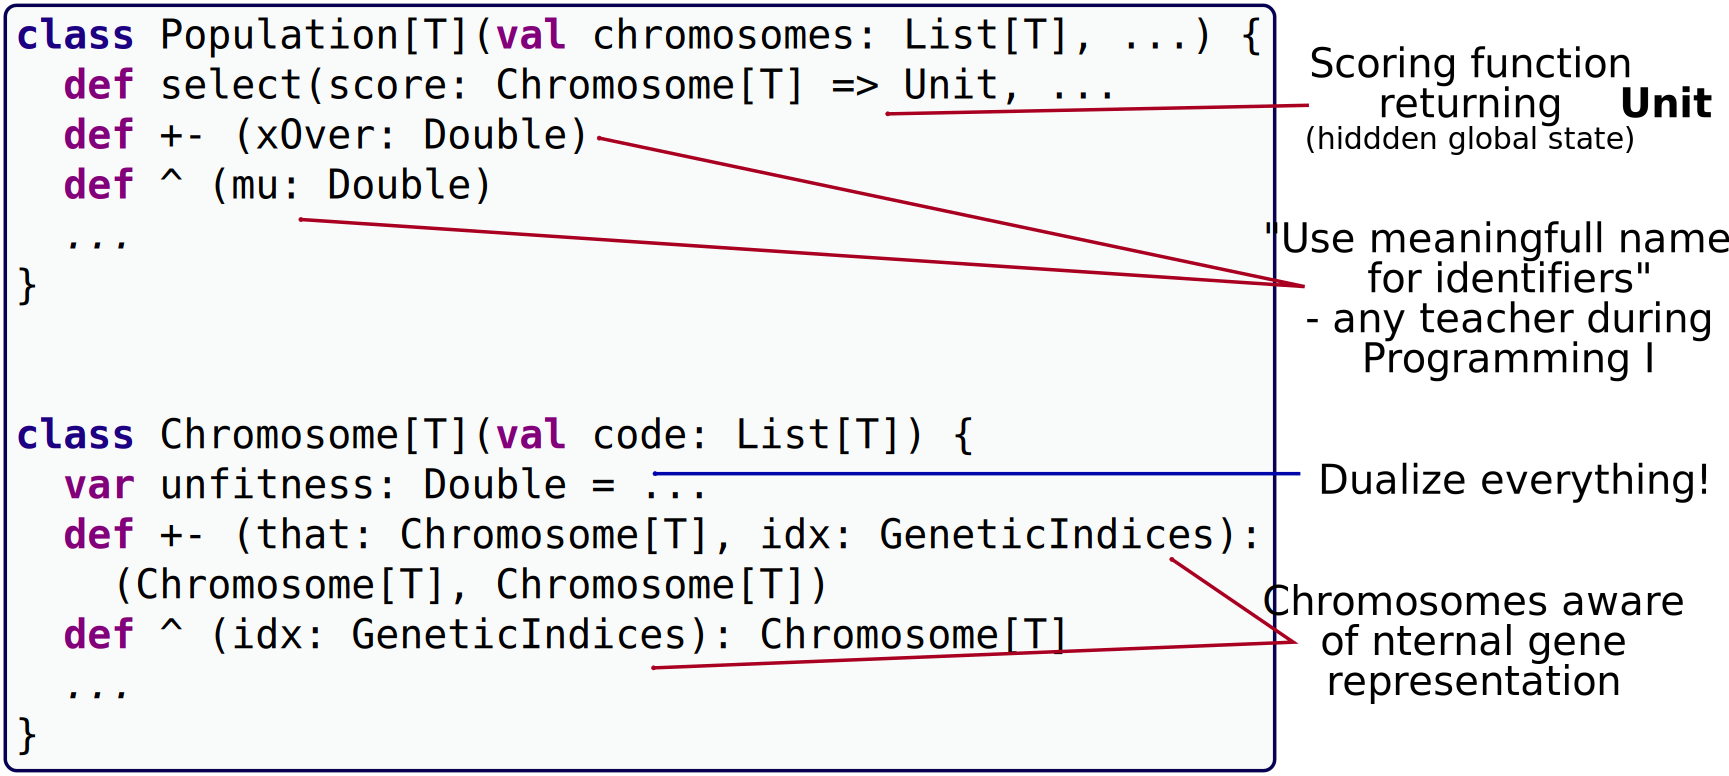
\includegraphics[width=0.9\textwidth]{images/sfml}
  \end{center}
  \footnotesize{
    \begin{thebibliography}{99}
      \bibitem[Label5, 2014]{key5} Patrick R. Nicolas
      \newblock Scala for Machine Learning
    \end{thebibliography}
  }
\end{frame}



%%%%%%%%%%%%%%%%%%%%%%%%%%%%%%%%%%%%%%%%%%%%%%%%%%%%%%%%%%%%%%%%%%%%%%%%
% Conclusion
\begin{frame}{The End -- Thank You}
  \begin{block}{Conclusion}
    The goal of stressing Scala's features to develop a genetic algorithms
    package was achieved:
    \begin{itemize}
      \item[\Checkmark] both greedy and genetic algorithms
      \item[\Checkmark] flexible, stable code
      \item[\Checkmark] programming strategies supported by
                        theoretical and practical considerations
      \item[\XSolidBrush] Scala is not as common as other alternatives (Java, C++)
      \item[\XSolidBrush] still open questions (Scala vs OCaml, binary methods...)
    \end{itemize}
  \end{block}
\end{frame}

\end{document}